\documentclass[a4paper]{article}
\usepackage[ngerman]{babel}
\usepackage[T1]{fontenc}
\usepackage[utf8]{inputenc}
\usepackage{textcomp}
\usepackage{geometry}
\geometry{ left=2cm, right=2cm, top=2cm, bottom=4cm, bindingoffset=5mm}
\usepackage{graphicx}
\usepackage{xcolor}
\usepackage{hyperref}
\date{}
\author{}
\usepackage{fancyhdr}
\pagestyle{fancy}
\fancyhf{}
\fancyhead[R]{3141241 - Jamie Ullerich \\ 2892258 - Gerhard Breul \\ 2973140 - Felix Bühler}
\fancyhead[L]{Information Visualisation and Visual Analytics \\ WS 2019/20 }
\renewcommand{\headrulewidth}{0.5pt}
\usepackage{tikz}
\usetikzlibrary{calc}
\usepackage{amsmath}



\title{\textbf{Assignment 3}}

\begin{document}
\maketitle 
\thispagestyle{fancy}

\section*{Task 1 - Lie Factor}
\subsection*{1.1}
\begin{align*}
\text{Lie Factor}&= \dfrac{\text{Size of effect in graphic}}{\text{Size of actual effect in data}}\\
ratio &= 590px / 275px = 2.145\\
Area_{Poland} &= 590px * 275px = 162,250px\\
Area_{Italy} &= 405px * (405px / 2.145) = 405px * 189px = 76,545px\\
Area_{Spain} &= 200px * (200px / 2.145) = 200px * 93px = 18,600px\\
\text{Lie Factor}_{\text{Poland, Italy}} &= \dfrac{\frac{162,250px - 76,545px}{76,545px}}{\frac{4431 - 3480}{3480}} = 4.097\\
\text{Lie Factor}_{\text{Poland, Spain}} &= \dfrac{\frac{162,250px - 18,600px}{18,600px}}{\frac{4431 - 2468}{2468}} = 9.71\\
\text{Lie Factor}_{\text{Italy, Spain}} &= \dfrac{\frac{76,545px - 18,600px}{18,600px}}{\frac{3480 - 2468}{2468}} = 7.597
\end{align*}
lie factor should have a value between 0.95 and 1.05, otherwise a great distortion is detected.

\subsection*{1.2}
The lie factor is for both exactly the same, because the used doors have the same dimensions. In the first picture there is no background and therefore the lie factor can easily be spotted. In the second one the background adds perspective, which in turn makes the actual values blur.

\section*{Task 2 - Gestalt Principles}
\begin{enumerate}
	\item[a)]
	Law of Continuity: it is possible to read the two words ''Coca'' and ''Cola'', even though they overlap. 
	Law of Connectedness: the two words are connected with lines and therefore it is obvious which letters from the word. 
	\item[b)]
	Law of Closure: there is no outline in this logo, but we can read the letters IBM. The vertical lines are ending where the outline of the letter would be and therefore it seems as if the contours are closed.  
	\item[c)] 
	Law of Similarity: the rectangle is perceived as one group since it is made of the same objects which share the same features. 
	It is also possible to read the word ''SUN'' on the edges of the rectangle, even though it consists only of the letter ''U''.
	\item[d)] 
	Law of Proximity: the U is composed of different shapes and smaller objects, but it is still clear, that this forms the letter U. 
\end{enumerate}

\section*{Task 3 - Pre-Attentive Processing}
\begin{enumerate}
	\item[1)]
	Pre-attentive processing can be utilized by highlighting the sought-after word in a different color. This will make it instantly recognizable among the black and white text.\\
	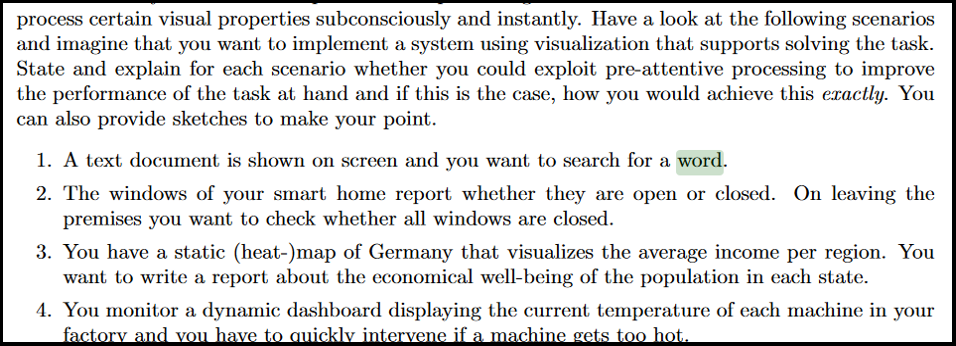
\includegraphics[width=\linewidth]{markedText1.png}
	
	\item[2)]
	Pre-attentive processing can be utilized by displaying an open window with a different color and orientation. This way, an open window is instantly recognizable\\
	
	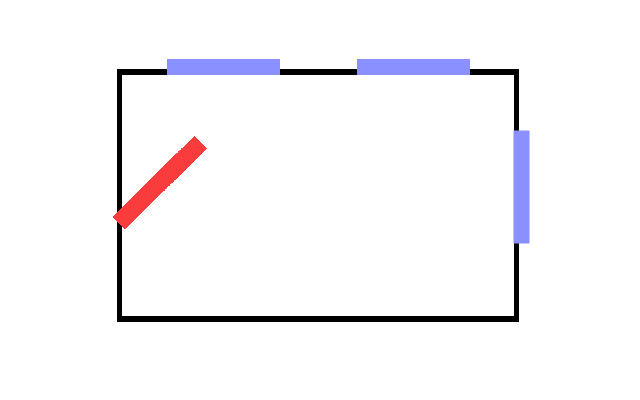
\includegraphics[width=\linewidth]{openWindow.png}
	
	\item[3)]
	For this task, exploiting pre-attentive processing is more difficult than for the previous tasks. One example oculd be to make every region above a certain income threshold visually distinct by coloring them in a noticably different color. This, however, would lose some information compared to a coloring based on a spectrum.
	
	\item[4)]
	By having each machine represented by a colored icon, it is possible to exploit pre-attentive processing to enhance performance in this task. Once a machine is close to overheating, the corresponding symbol turns from green/blue to yellow. When it starts to overheat, the icon turns red. Additional visual highlights such as a box around it or a flashing effect could be imagined as well.
	
	\item[5)]
	For each test result that is outside of normal values, the number describing it is highlighted by being written in bold or underlined numbers. For extreme cases, these values could even be shown in a different color.
	
\end{enumerate}

	
\end{document}
